\documentclass[11pt,a4paper]{article}
\usepackage[margin=27mm]{geometry}
\usepackage{fontspec,booktabs,array,hyperref,graphicx}
\setmainfont{STIXGeneral}
\setlength{\parindent}{0pt}\setlength{\parskip}{5pt}
\begin{document}
\begin{center}{\Large Complete manuscript comparison}\\[3pt]
Overview v15: two-source Representation\end{center}
There are 18 topics and 48 recovered originals among 106 accessible originals; 58 remain pending and 55 earlier indexed originals remain archived. Representation now includes L126 alongside F010. The other 17 topic records and 46 individual records retain their exact v14 boundaries. The complete Representation factor is $60,472/82,152=0.736099$: written expansion, not achieved whole-topic compression.

For each topic the complete written factor is $\sum_i c(S_i)/(c(U)+\sum_i c(A_i))$. Whole common theory and all complete applications are paid once within that topic. Each row retains its independently adopted nonwhitespace-character coordinate; there is no cross-topic discount, pooled factor or inferred minimum proof complexity. Concrete software listings are excluded on both sides. Proof and mathematical algorithm prose remain counted.
\begin{center}\small\begin{tabular}{lrrrrr}\toprule
Topic & Originals & Sources & Common & Applications & Factor\\\midrule
A & 8 & 246,570 & 66,140 & 110,576 & 1.395 \\
B & 5 & 124,906 & 44,905 & 69,265 & 1.094 \\
C & 5 & 118,433 & 30,437 & 61,248 & 1.292 \\
D & 3 & 47,894 & 15,632 & 29,855 & 1.053 \\
E & 5 & 140,286 & 57,473 & 32,337 & 1.562 \\
F & 2 & 69,825 & 15,876 & 27,398 & 1.614 \\
G & 2 & 73,199 & 30,928 & 85,207 & 0.630 \\
Representation & 2 & 60,472 & 36,715 & 45,437 & 0.736 \\
Chamber & 2 & 34,177 & 15,199 & 21,254 & 0.938 \\
Matching & 1 & 37,951 & 16,732 & 17,168 & 1.119 \\
ChiralEnumeration & 1 & 27,594 & 8,831 & 23,171 & 0.862 \\
Operations & 3 & 200,630 & 58,215 & 100,379 & 1.265 \\
Gluing & 1 & 27,081 & 28,416 & 11,565 & 0.677 \\
RankContraction & 1 & 15,530 & 6,937 & 10,555 & 0.888 \\
LocallyProjective & 2 & 26,490 & 25,498 & 11,966 & 0.707 \\
MathieuCensus & 1 & 13,736 & 5,516 & 35,862 & 0.332 \\
RankAugmentation & 1 & 33,604 & 13,904 & 14,096 & 1.200 \\
Mixes & 3 & 156,570 & 34,757 & 68,693 & 1.513 \\
\bottomrule\end{tabular}\end{center}
The \href{topics.csv}{18-topic CSV} and \href{applications.csv}{48-original CSV} preserve exact fractions, complete component lengths and historical observations. Factors below one remain visible. The source maps and separate admissions determine the recovered principal contracts; this numerical overview adds no separate proof or question credit.
\newpage
\section*{Individual comparisons: first 24 originals}
After acquiring the \emph{whole} common theory and all actual required mathematical, computational and data premises, the conditional factor is $c(S_i)/c(A_i)$. The complete local application or companion bundle remains charged.
\begin{center}\small\begin{tabular}{llrrr}\toprule
Original & Topic & Source & Application & Factor\\\midrule
L032 & A & 16,558 & 8,228 & 2.012 \\
L034 & A & 21,433 & 5,801 & 3.695 \\
F016 & A & 43,983 & 15,436 & 2.849 \\
F013 & A & 25,562 & 6,241 & 4.096 \\
L035 & A & 51,019 & 14,514 & 3.515 \\
N009 & A & 36,824 & 28,130 & 1.309 \\
L128 & A & 18,424 & 8,825 & 2.088 \\
L012 & A & 32,767 & 23,401 & 1.400 \\
N001 & B & 14,519 & 7,371 & 1.970 \\
N003 & B & 17,780 & 9,155 & 1.942 \\
N008 & B & 18,009 & 11,132 & 1.618 \\
L030 & B & 22,704 & 12,286 & 1.848 \\
L040 & B & 51,894 & 29,321 & 1.770 \\
L088 & C & 13,166 & 11,311 & 1.164 \\
N013 & C & 27,361 & 15,815 & 1.730 \\
L108 & C & 12,849 & 10,075 & 1.275 \\
F014 & C & 20,577 & 6,962 & 2.956 \\
L068 & C & 44,480 & 17,085 & 2.603 \\
L066 & D & 20,916 & 10,989 & 1.903 \\
L074 & D & 20,661 & 13,367 & 1.546 \\
L104 & D & 6,317 & 5,499 & 1.149 \\
L079 & E & 21,212 & 1,858 & 11.417 \\
L083 & E & 20,904 & 2,922 & 7.154 \\
L021 & E & 29,594 & 14,452 & 2.048 \\\bottomrule\end{tabular}\end{center}
Representation pays the complete 13-page shared theory and both applications of four and twelve pages: \[36,715+10,985+34,452=82,152.\] The sources total $25,348+35,124=60,472$ characters. The primary remains calibrated selected text, NFC, excluding whitespace. The finite-normal-pair existence proof is now fully in the common paper; no sibling application is free.

After paying whole U and retained premises, F010 has factor $2.307510$; L126 has factor $1.019505$. These conditional reuse figures do not undo the expansion of the full proof. L126 additionally requires the complete graph certificate and full 19,326-byte JSON; nine validation programs are optional.
\newpage
\section*{Individual comparisons: remaining 24 originals}
\begin{center}\small\begin{tabular}{llrrr}\toprule
Original & Topic & Source & Application & Factor\\\midrule
L056 & E & 15,871 & 4,144 & 3.830 \\
L043 & E & 52,705 & 8,961 & 5.882 \\
L014 & F & 25,574 & 11,504 & 2.223 \\
L007 & F & 44,251 & 15,894 & 2.784 \\
L009 & G & 49,891 & 23,544 & 2.119 \\
L092 & G & 23,308 & 61,663 & 0.378 \\
F010 & Representation & 25,348 & 10,985 & 2.308 \\
L126 & Representation & 35,124 & 34,452 & 1.020 \\
L008 & Chamber & 20,159 & 7,571 & 2.663 \\
N016 & Chamber & 14,018 & 13,683 & 1.024 \\
F015 & Matching & 37,951 & 17,168 & 2.211 \\
L028 & ChiralEnumeration & 27,594 & 23,171 & 1.191 \\
N005 & Operations & 122,002 & 49,595 & 2.460 \\
N006 & Operations & 55,740 & 38,479 & 1.449 \\
N007 & Operations & 22,888 & 12,305 & 1.860 \\
L010 & Gluing & 27,081 & 11,565 & 2.342 \\
L037 & RankContraction & 15,530 & 10,555 & 1.471 \\
L084 & LocallyProjective & 2,071 & 4,857 & 0.426 \\
L095 & LocallyProjective & 24,419 & 7,109 & 3.435 \\
L073 & MathieuCensus & 13,736 & 35,862 & 0.383 \\
L020 & RankAugmentation & 33,604 & 14,096 & 2.384 \\
F005 & Mixes & 57,753 & 31,077 & 1.858 \\
L016 & Mixes & 35,506 & 15,125 & 2.348 \\
F007 & Mixes & 63,311 & 22,491 & 2.815 \\\bottomrule\end{tabular}\end{center}
The Representation source contract retains six F010 blocks and 31 L126 dispositions, with finite-field/small-case corrections and an explicit chamber-connectivity hypothesis for splitting. The broader Section 6.2 and Section 8 programmes remain unresolved. The exact source editions and independent proof/input/numerical records are linked by its admission.

The 16-page program appendix prints all ten programs. Its 35,723 characters and the raw programs' 34,823 are alternatives, never added twice. The mandatory JSON contributes 19,315 raw nonspace characters separately; it is not replaced by the appendix. Two current helpers and four partial Lean modules/22 declarations are separate inventories. Neither full source is formalized.

Historical software, retained external proofs, complete graphics and full formalization costs remain unknown. All software-inclusive and pooled factors are null. Operations retains its separate text-only sensitivity; expanded E retains its accepted source qualifications and the source's Magma/$L_2$-quotient attribution. Prior overviews remain historical records.
\newpage
\section*{Whole topics}
Grey bars show the complete original manuscript text in each row's adopted coordinate. Replacement bars stack the entire common theory and all applications. The axis starts at zero; the tables give the ratios.
\begin{center}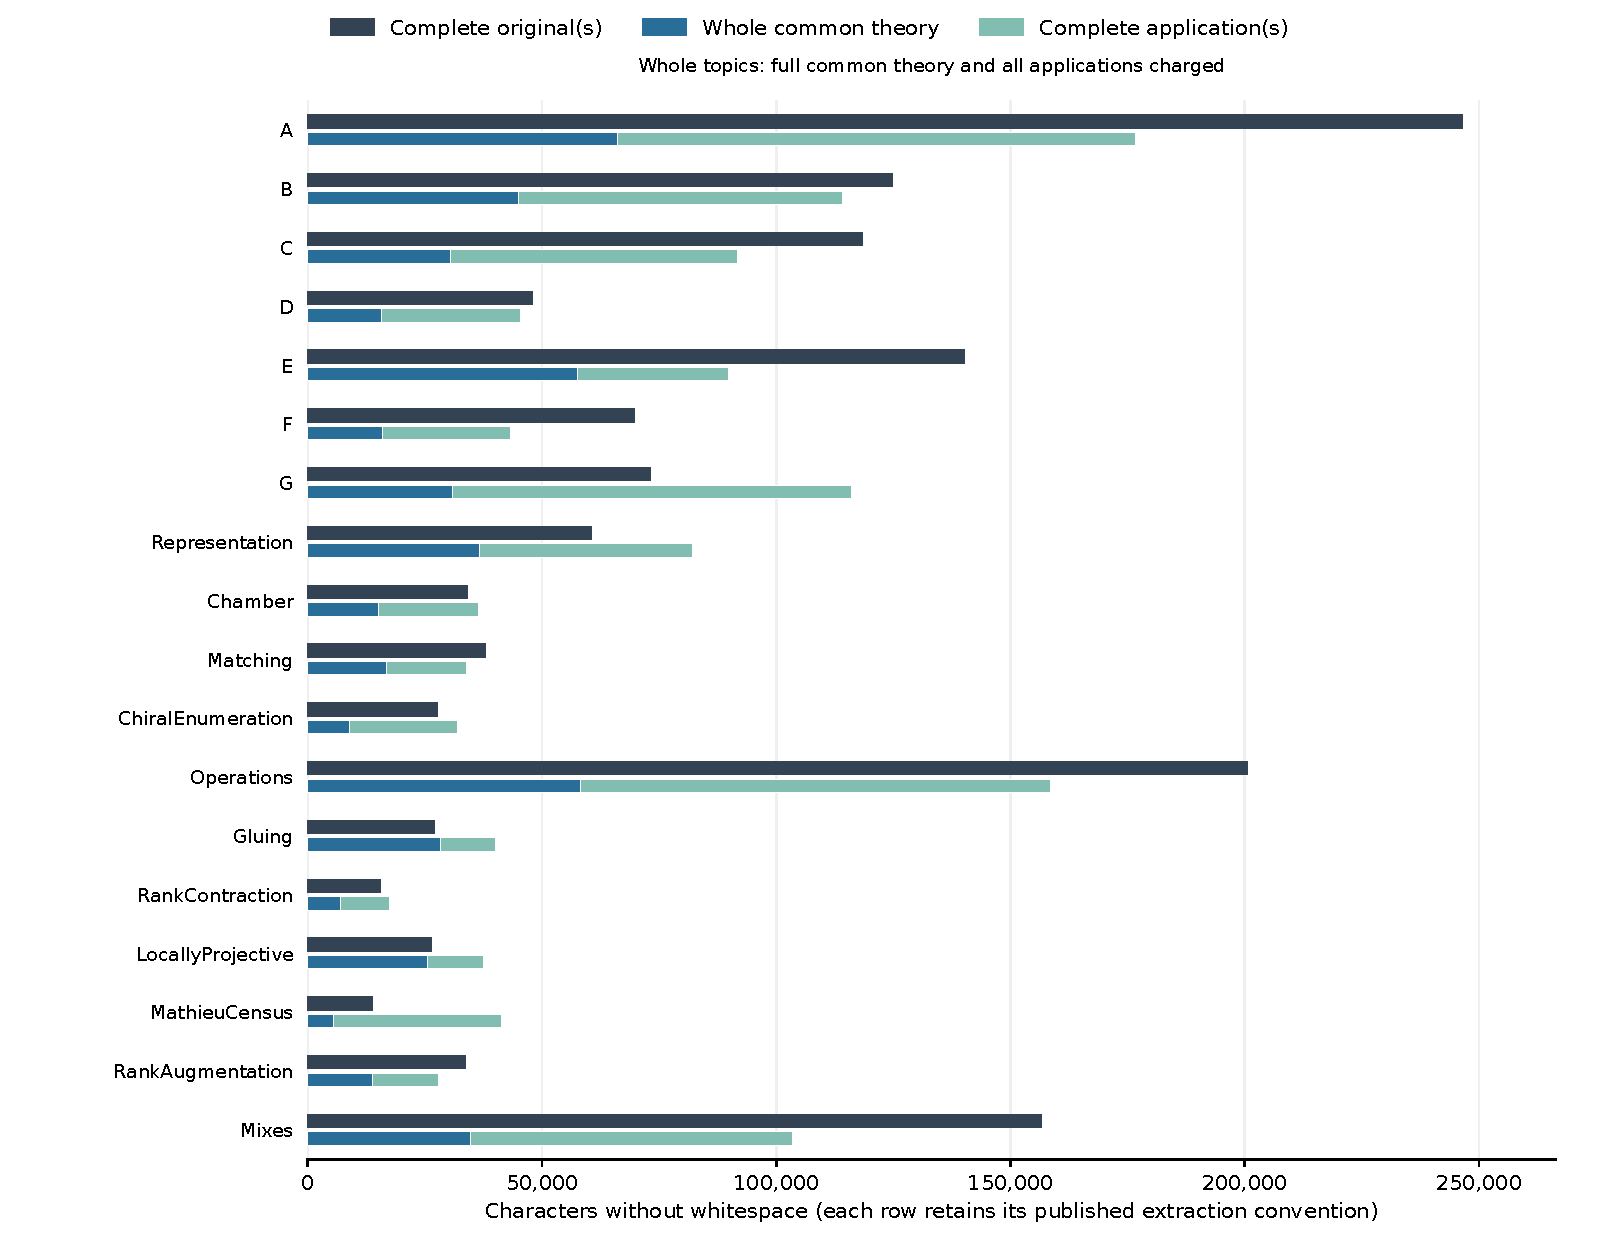
\includegraphics[width=\linewidth]{whole_topics.pdf}\end{center}
The 54 bars account for all 18 topics. No necessary finite certificate or external premise becomes optional merely because software and retained external proof costs are outside the manuscript coordinate.
\newpage
\section*{Conditional lengths: first 24 originals}
Whole common theory and required premises are acquired in advance. Grey and teal bars compare complete source and local application text; the whole-topic table still pays the common theory.
\begin{center}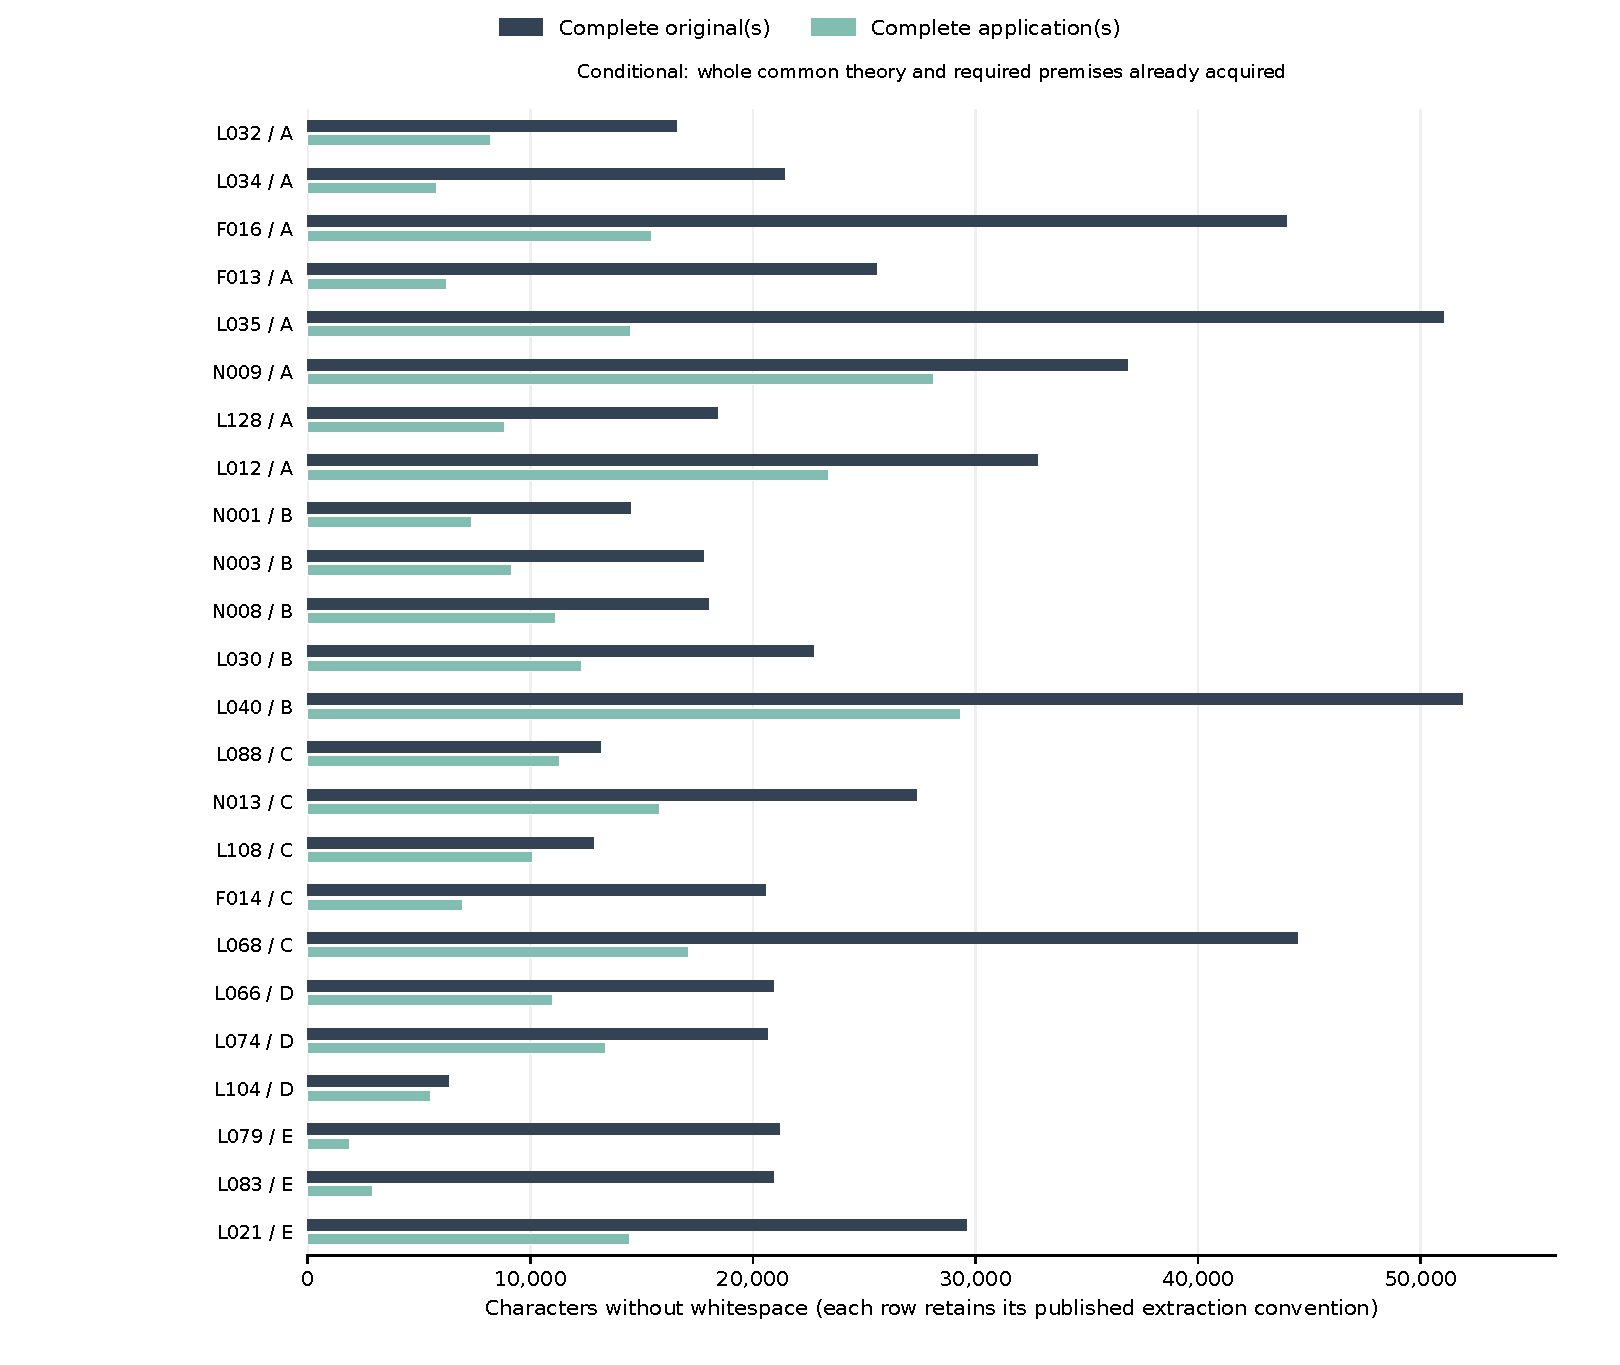
\includegraphics[width=\linewidth]{conditional_1.pdf}\end{center}
\newpage
\section*{Conditional lengths: remaining 24 originals}
All complete companion papers remain charged. The source order is documentary, not an optimal acquisition order or a claimed sawtooth.
\begin{center}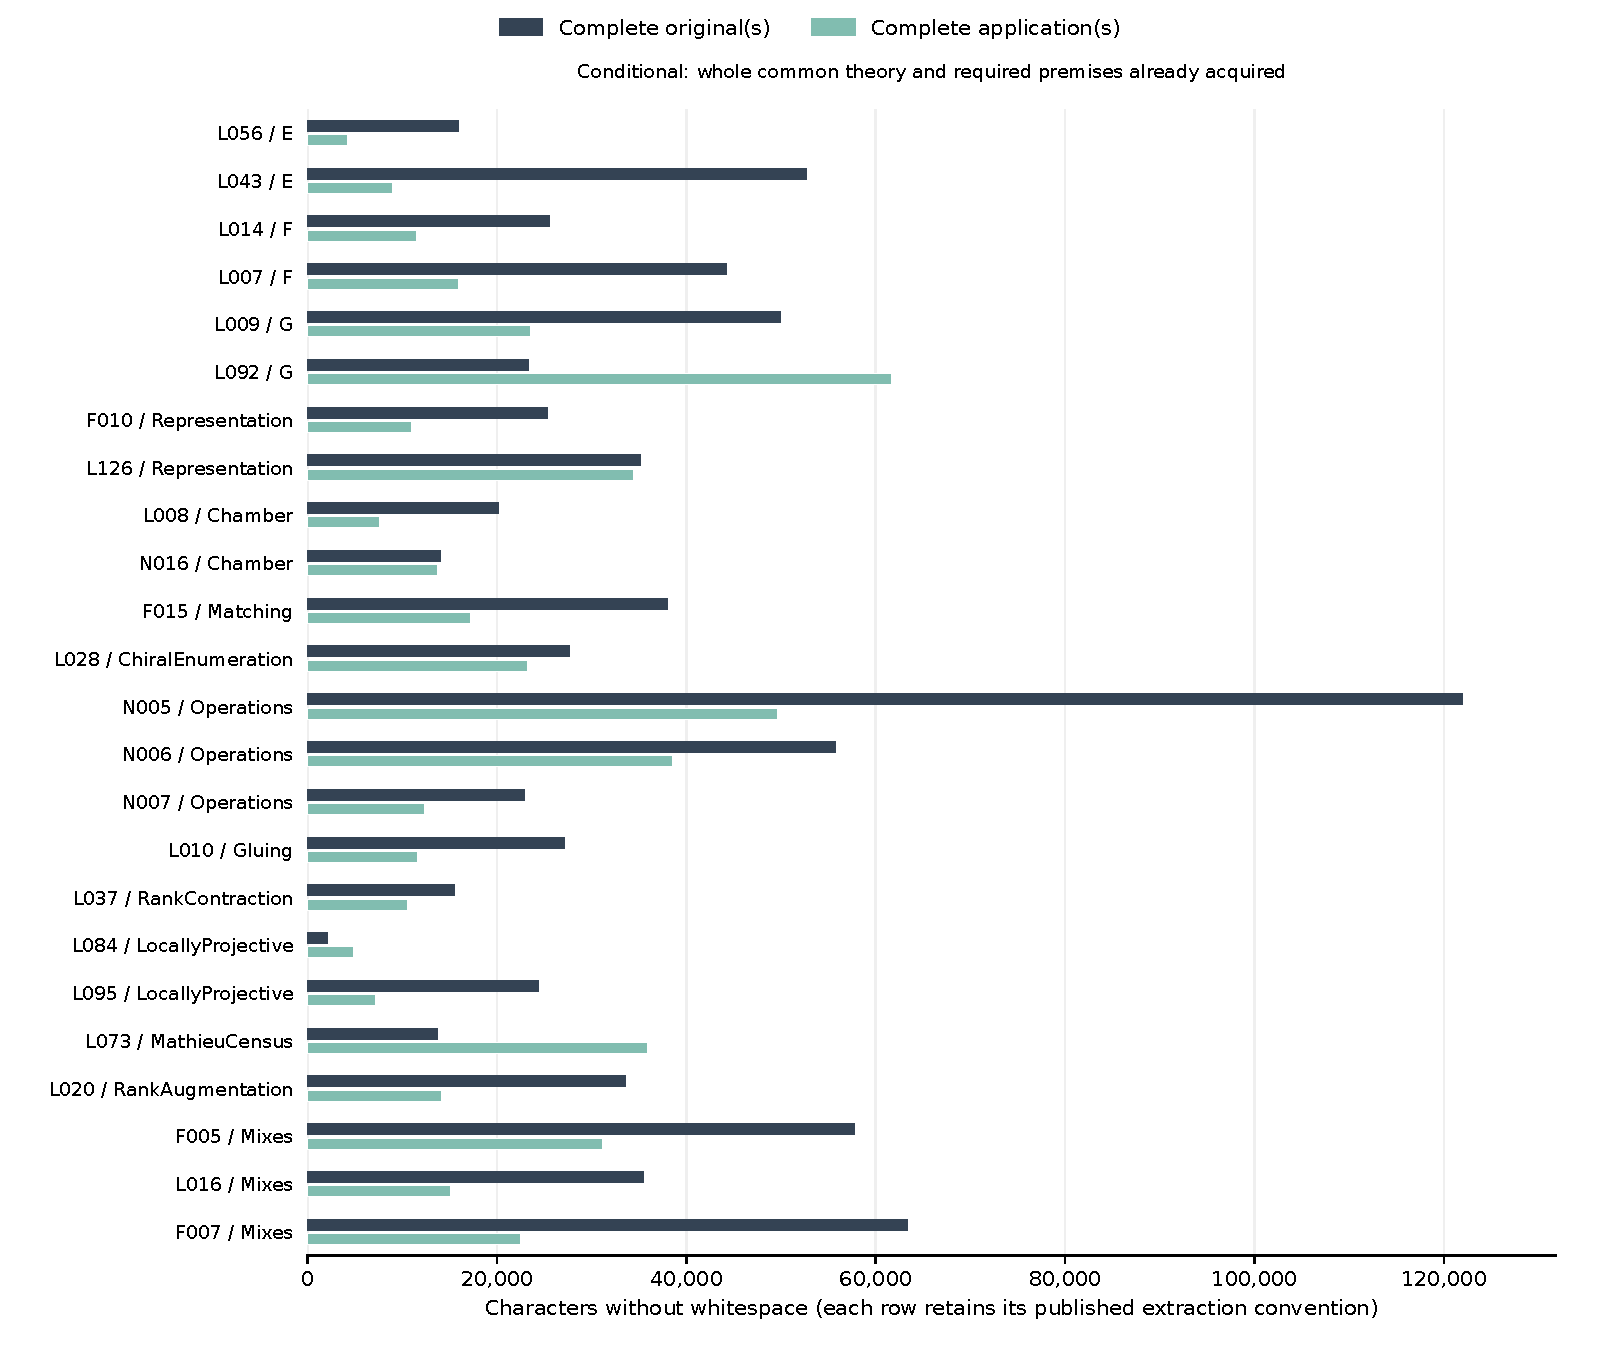
\includegraphics[width=\linewidth]{conditional_2.pdf}\end{center}
This edition supplies 66 exact written comparisons and 150 plotted bars. The active programme remains 106 originals, with 48 recovered and 58 pending. Only L126 is newly reflected from its separate scientific admission; F010 was already admitted. No new question or priority claim is made.
\end{document}
